\newpage
\section{Diseño del Sistema}

\subsection{MOD 1}
\label{sec5.1.}
\subsubsection{Diseño Detallado del MOD 1}
\textbf{* Diseño de R1 y R2:}\par
Según RP1 (asumiendo que la impedancia del condensador es despreciable) se calcula la equivalencia Thévenin total mediante el principio de superposición, calculando inicialmente el Thévenin alterno:\par 
\begin{figure}[h!]
    \Centering
    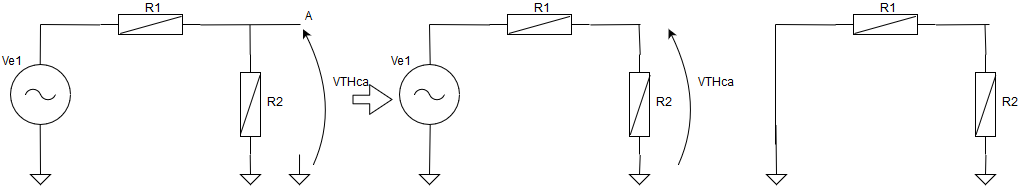
\includegraphics[scale=0.45]{Imagenes/6DisenoSistema/VTHcaMOD1.png}
    \caption{Voltaje Thevenin Alterno MOD 1}
	\label{fig:figure6}
\end{figure}
Para calcular el Voltaje de Thevenin, es necesario hacer un divisor de tensión en R2:\par 
\begin{center}
$\frac{Ve1 * R2}{R2 + R1} = VTHca$ \hspace{0.5cm} $\Rightarrow$\hspace{0.5cm} $\frac{0.1 * R2}{R2 + R1} = 0.05$ \hspace{0.5cm}$\Rightarrow$ \hspace{0.5cm}$0.05(R2 - R1) = 0$\\[0.5cm]
$\therefore R1  = R2$
\end{center}
Aquí se obtiene desde la información de RP3 que para que se cumpla lo solicitado las resistencias R1 y R2 deben ser iguales.\par

Para calcular la Red relajada de Thevenin apagamos la fuente de voltaje alterno:\par 
\begin{center}
 $\frac{R1 * R2}{R2 + R1} = ZTH_{ca}$\hspace{0.5cm} $\Rightarrow$\hspace{0.5cm} $\frac{R * R}{R + R}\geq 85 [\Omega]$\hspace{0.5cm} $\Rightarrow$ \hspace{0.5cm}$\frac{R}{2} \geq 85[\Omega]$\\[0.5cm]
$\therefore R\geq 170[\Omega]$   
\end{center}
Con los datos de RP3, buscamos el cumplimiento de los requisitos, obteniendo como resultado que tanto R1 como R2 deben ser mayores a 170 $[\Omega]$.\\[0.2cm] 

Por otro lado según RP3 cuando conectamos los módulos uno y dos debemos lograr que el punto de operación de nuestro diodo(1n4148) sea (0.72 [v],0.018 [A]), para ello analizamos el siguiente esquema:\par 
\begin{figure}[h!]
    \Centering
    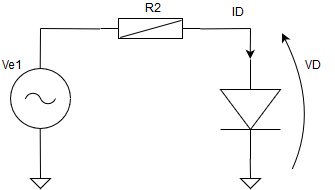
\includegraphics[scale=0.45]{Imagenes/6DisenoSistema/DISENORP2.png}
    \caption{Circuito diodo 1N4148}
	\label{fig:figure6}
\end{figure}

\newpage

Por LVK y tercer postulado podemos determinar el valor de R2:\par 
\[Ve2 = VR2 + VD \Rightarrow Ve2 = R2*IR2 + VD\Rightarrow R2 = \frac{Ve2 - VD}{IR2}\Rightarrow R2 = \frac{6.7[V]-0.72[V]}{0.018[A]}\]
\[\therefore R2 = 332.2[\Omega]\]

Por comodidad a la hora de formar el circuito definiremos tanto R2 como R1 con el valor de 330$[\Omega]$.\par 

La gráfica del diodo ID = f(VD) se obtendrá en el laboratorio, lo cual será especificado en la sección de estrategias de pruebas.\\[0.5cm]



\textbf{* Diseño de C1:}\\[0.1cm]
Según lo solicitado en RP2, la impedancia de C1 debe ser despreciable respecto a la resistencia vista por los terminales de salida, o bien, su resistencia equivalente Thévenin. Podemos notar que la impedancia más baja Thévenin que podemos obtener está dada por el mínimo de $ZTH_{ca}$; 170 $[\Omega]$ en este caso.
Por ende la impedancia del condensador (Zc1) dada por $\frac{1}{C}$ , debe cumplir :
Zc1 $<<$ 170 $[\Omega]$, tomamos el criterio de que 10 veces menor (mínimo) será un valor despreciable. Por esto, teniendo en cuenta que estamos trabajando con una frecuencia 3[KHz], el condensador fácilmente funcionará de la manera que necesitamos. Luego de dicho análisis definiremos $C1 = 10[\mu F]$.\par 


\subsubsection{Estrategias de Prueba MOD 1}
En el laboratorio, se comenzará montando el Módulo 1, según los valores de los componentes obtenidos en la subsección anterior. Además, se utilizará el generador de señales para obtener el voltaje Ve1, programado a 3[Khz] de frecuencia y 0.1 [V] de amplitud, centrada en 0, por otro lado, usaremos la fuente de voltaje continua para recrear la fuente Ve2, configurada a 6,7 [V]
En laboratorio, para ratificar que el sistema es lineal, lo cual podemos esperar, ya que utilizamos componentes lineales (pasado su transciente) y la suma de las fuentes se mantiene para diferentes valores de entrada se realizará una tabla donde se analizarán los valores de entrada y salida, realizando 4 incrementos discretos para la amplitud de cada fuente, y anotando los respectivos valores de las señales de entrada y salida.
 Comprobaremos además que los valores del condensador son despreciables analizando la existencia de desfase entre la entrada y salida por medio del osciloscopio.


\subsection{MOD 2}
\label{sec5.2.}
\subsubsection{Diseño Detallado del MOD 2}
\textbf{* Diseño de R4:}\\[0.2cm]
Dado RP5 y sabiendo que la resistencia dinámica del diodo en el punto indicado en RP4 es $RD = \frac{0.72[V]}{0.018[A]}$ podemos determinar que:\\[-0.2cm]

\begin{center}
$R4 \geq 10* RD$ \hspace{0.5cm} $\Rightarrow$ \hspace{0.5cm}$R4 \geq 10*40[\Omega]$\hspace{0.5cm}$\Rightarrow$\hspace{0.5cm}$\therefore R4 \geq 400[\Omega]$
\end{center}

\textbf{* Diseño de C2:}\\[0.2cm]
Según lo solicitado en RP2, la impedancia de C2 debe ser despreciable respecto a la resistencia vista por los terminales de salida, o bien, su resistencia equivalente Thévenin. Podemos notar que la impedancia más baja Thévenin que podemos obtener está dada por el mínimo de $ZT_{ca} << 170 $ $[\Omega]$ en este caso.
Por ende la impedancia del condensador (Zc1) dada por $\frac{1}{C}$ , debe cumplir :
$Zc1 << 170$ $[\Omega]$  , tomamos el criterio de que 10 veces menor (mínimo) será un valor despreciable. Por esto, teniendo en cuenta que estamos trabajando con una frecuencia 3[KHz], el condensador fácilmente funcionará de la manera que necesitamos. Luego de dicho análisis definiremos $C2 = 10[\mu F]$.\\[0.2cm]

\textbf{* Determinar factor k:}\\[0.2cm]
Para determinar K solo hace falta sacar el equivalente thevenin continuo, para luego compararlo con su expresión matemática relacionada.\par

\begin{figure}[h!]
    \Centering
    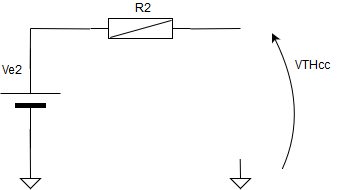
\includegraphics[scale=0.45]{Imagenes/6DisenoSistema/TheveninContinuo.png}
    \caption{Thevenin Voltaje Continuo MOD 1}
	\label{fig:figure6}
\end{figure}





Podemos decir que $VTH_{cc} = Ve2$ , por lo que según la ecuación de RF1:\par 
\begin{center}
    $Va = Ve2 + kVe1 \Rightarrow 6.75 [V] = 6.7 [V] + k +(0.1[V]) \Rightarrow \therefore k = 0.5$\par
    $Va = Ve2 + kVe1 \Rightarrow 6.65 [V] = 6.7 [V] + k +(-0.1[V]) \Rightarrow \therefore k = 0.5$\par
\end{center}
Se concluye que k como coeficiente tiene un valor fijo de 0.5.\\[0.2cm] 

\textbf{* Determinar factor n:}\\[0.1cm]

Para determinar n necesitamos una expresión que relación Ve1 con Vs1, en donde influya Ve2. Por lo visto anteriormente Ve2 esta directamente relacionado con la resistencia dinámica del diodo, como resultado si obtenemos un thevenin alterno para Vs1 nos queda la siguiente expresión:\par 
\begin{center}
    $n = \frac{Vs1}{Ve1}$ $\Rightarrow $ $n = \frac{Vs1 *\frac{330 // RD // 1K}{330 + 330// RD // 1K}}{Vs1}$ $\Rightarrow$ $n = \frac{253.8*RD}{330 + 253.8RD}$
\end{center}

Por otro lado tenemos la relación de Ve2 con VD:\Rpar 
\begin{center}
    $Ve2 = ID*R2 + VD$
\end{center}
Donde a su vez, si vemos la gráfica de ID =f(VD) podemos calcular RD implícitamente. Calculando RD podemos determinar un valor para n.\par







\subsubsection{Estrategias de Prueba MOD 2}
Primeramente comenzaremos analizando experimentalmente la curva característica de nuestro diodo, por medio de una tabla de valores. Realizaremos incrementos discretos de corriente mediante la variación de una resistencia (probablemente con ayuda de un potenciómetro), con una fuente fija. Con esto podremos predecir de manera más exacta los resultados ya que obtendremos su característica real.
Luego para probar el funcionamiento y la validez de los valores de componentes obtenidos a través del análisis matemático, según la sección de requisitos de prueba, realizaremos la construcción de circuito en el laboratorio, prestando principal atención en que los valores de salida del módulo 2 correspondan según lo especificado por la sección 4.2, principalmente comprobando el valor del punto de operación del diodo por otro lado verificar que la señal alterna de salida sea atenuada, al variar el valor de la fuente continua como se podría esperar.
Lo anterior será medido con ayuda de los Osciloscopios y Multímetros ocupados en el laboratorio.
